\documentclass[10pt, table, dvipsnames,xcdraw, handout]{beamer}
\usetheme[progressbar=frametitle]{metropolis}
\usepackage{appendixnumberbeamer}
\usetikzlibrary{arrows.meta, positioning, quotes}
\usepackage[shortlabels]{enumitem}
\usepackage{xcolor}
\usepackage{mathtools}
\usepackage{dsfont}

\usepackage{caption}


\usepackage{cancel}

\newcommand\hcancel[2][black]{\setbox0=\hbox{$#2$}%
\rlap{\raisebox{.45\ht0}{\textcolor{#1}{\rule{\wd0}{1pt}}}}#2} 


\usepackage{booktabs}
\usepackage[scale=2]{ccicons}

\usepackage{pgfplots}
\usepgfplotslibrary{dateplot}

\usepackage{xspace}
\newcommand{\themename}{\textbf{\textsc{metropolis}}\xspace}
\newcommand{\cb}{\cellcolor{blue!25}}


% Notation:
\newcommand{\cT}{\ensuremath{\mathcal{T}}}
\newcommand{\cD}{\ensuremath{\mathcal{D}}}
\newcommand{\cX}{\ensuremath{\mathcal{X}}}
\newcommand{\cY}{\ensuremath{\mathcal{Y}}}
\newcommand{\cZ}{\ensuremath{\mathcal{Z}}}
\newcommand{\cH}{\ensuremath{\mathcal{H}}}
\newcommand{\cG}{\ensuremath{\mathcal{G}}}

\newcommand{\bR}{\ensuremath{\mathbb{R}}}
\newcommand{\bN}{\ensuremath{\mathbb{N}}}
\newcommand{\bP}{\ensuremath{\mathbb{P}}}
\newcommand{\bT}{\ensuremath{\mathbb{T}}}
\newcommand{\bL}{\ensuremath{\mathbb{L}}}

\newcommand{\bfX}{\ensuremath{\mathbf{X}}}
\newcommand{\bfY}{\ensuremath{\mathbf{Y}}}
\newcommand{\bfy}{\ensuremath{\mathbf{y}}}
\newcommand{\bfD}{\ensuremath{\mathbf{D}}}

\def\layersep{2.5cm}

% Tikz seys
\tikzset{cross/.style={cross out, draw, 
         minimum size=2*(#1-\pgflinewidth), 
         inner sep=0pt, outer sep=0pt}}

\title{Machine Learning I}
\subtitle{Lecture 17: Boosting, Bagging and Bootstrapping}
% \date{\today}
\date{}
\author{Nathaniel Bade}
\institute{Northeastern University Department of Mathematics}
% \titlegraphic{\hfill\includegraphics[height=1.5cm]{logo.pdf}}

\begin{document}

\maketitle

\begin{frame}{Table of contents}
  \setbeamertemplate{section in toc}[sections numbered]
  \tableofcontents[hideallsubsections]
\end{frame}


%%%%%%%%%%%%%% Slidshow Start %%%%%%%%%%%%%% 


%Notes: 4 kinds of clusering: Centroid based/kmeans, connecctivity based, density based, distribution based. 
%
% What metrics can we use to evalaute scattering? (internal) Scatter crieteria, silloett coeffcient, (external) mutial information, 
% 
%
% Association rules and merket basket analysis. 
%
%
%
%

\section{Introduction to Boosting}

\begin{frame}[fragile]{Introduction to Boosting}
  \begin{minipage}[t][0.5\textheight][t]{\textwidth}
	\centering \includegraphics[width=\textwidth]{L19Comitee.png} 
  \end{minipage}
  \vfill
\begin{minipage}[t][0.5\textheight][t]{\textwidth}
Boosting started as a theoretical question: Can a committee of fast learning, slightly-better-than-average algorithms combine to form an algorithm with strong predictive power? \pause\newline

 In 1990, Robert Schapire answer the theoretical question in the affirmative. Five years later, he produced with Yoav Freund a practical implementation called Adaboost.
\end{minipage}
\end{frame}




\begin{frame}[fragile]{Introduction to Boosting}
  \begin{minipage}[t][0.5\textheight][t]{\textwidth}
	\centering \includegraphics[height=.5\textheight]{L19BoostTraining1.png} 
  \end{minipage}
  \vfill
\begin{minipage}[t][0.5\textheight][t]{\textwidth}
Consider a two class problem, $\mathcal{Y} = \{-1,1\}$ with a vector space $\cX$ of features. Roughly, a weak classifier $G$ is one whose error rate is slightly better than random guessing. \pause\newline 

The key innovation in boosting algorithms is to fit each basis element \textbf{sequentually} instead of in paralllel. By sequentially applying weak classifiers to repeated modified version of the data, we can form a weighted sum of prediction classes. 
\end{minipage}
\end{frame}



\begin{frame}[fragile]{Introduction to Boosting}
  \begin{minipage}[t][0.5\textheight][t]{\textwidth}
	\centering \includegraphics[height=.5\textheight]{L19BoostTraining2.png} 
  \end{minipage}
  \vfill
\begin{minipage}[t][0.5\textheight][t]{\textwidth}
By sequentially applying weak classifiers to repeated modified version of the data, we can form a weighted sum of prediction classes,
$$
G(x) = \text{sign}\left( \sum_{m=1}^M\alpha_mG_m(x) \right)\,,
$$
where $\alpha_i$ are computed by the boosting algorithm.
\end{minipage}
\end{frame}



\begin{frame}[fragile]{Introduction to Boosting}
  \begin{minipage}[t][0.5\textheight][t]{\textwidth}
	\centering \includegraphics[height=.5\textheight]{L19BoostTraining2.png} 
  \end{minipage}
  \vfill
\begin{minipage}[t][0.5\textheight][t]{\textwidth}
At each step of the algorithm, the data points which are misclassified in step $m$ will be weighted more strongly in step $m+1$. \pause For regression boosting, this means at each step we fit the weighted residuals of the previous step. 
\end{minipage}
\end{frame}



\begin{frame}[fragile]{Lecture Overview}
  \begin{minipage}[t][0.5\textheight][t]{\textwidth}
	\centering \includegraphics[height=.5\textheight]{L19BoostTraining2.png} 
  \end{minipage}
  \vfill
\begin{minipage}[t][0.5\textheight][t]{\textwidth}
In this lecture, we will see that by combining high bias, easy to train classifiers, boosting produces strong, computationally efficient classifiers with well controlled bias/variance trade off. \pause Of course the cost is going to be interpretability. Boosting produces solidly ``blackbox'' classifiers. That said, at the end of the lecture we will discuss some ways we can understand these results. 
\end{minipage}
\end{frame}


\begin{frame}[fragile]{Lecture Overview}
  \begin{minipage}[t][0.5\textheight][t]{\textwidth}
	\centering \includegraphics[height=.5\textheight]{L19BoostTraining2.png} 
  \end{minipage}
  \vfill
\begin{minipage}[t][0.5\textheight][t]{\textwidth}
We will focus in this lecture on Adaboost, the first and most popular boosting algorithm. We will show both some theoretical results, as well as discussing practical fitting methodology. Finally, we follow ESLII and UML and look closely at boosted tree classifiers. 
\end{minipage}
\end{frame}


\section{Adaboost}

\begin{frame}[fragile]{Adaboost Algorithm: Setup}
Consider a two class problem, $\mathcal{Y} = \{-1,1\}$ with a vector space $\cX$ of features. Let $\cT = \{(x_i,y_i)\}$ be  training set of size $N$ and let $G_m(x)$, $m=1,\ldots, M$ be a sequence of weak classifiers. \pause 

Our goal is to produce a weighted majority vote classifier
$$
G(x) = \text{sign}\left( \sum_{m=1}^M\alpha_mG_m(x) \right)\,,
$$\pause
where the weights are chosen algorithmically. We will now take a moment to describe the sequential training for the Adaboost algorithm. 
\end{frame}




\begin{frame}[fragile]{Adaboost Algorithm}
\textbf{Adaboost algorithm:}

\begin{itemize}
\item[]Initialize weights $w_i = 1/N$\,.
\item[] For $m=1$ to $M$,
\begin{itemize}
\item[$(1)$] Fit a classifier $G_m(x)$ to the training data weighted by $w_i$.
\item[$(2)$] Compute the training error:
$$
\text{Err}_m = \frac{1}{\sum_{i=1}^N w_i} \sum_{i=1}^N w_i\, \mathds{1}(y_i \neq G(x_i))\,.
$$
\item[$(3)$] Compute $\alpha_m = \log((1-\text{Err}_m)/\text{Err}_m)$
\item[$(4)$] Update each weight to $w_i = w_i\cdot \exp\big[ \alpha_m \mathds{1}(y_i \neq G(x_i)) \big]$, $i=1,\ldots, N$.
\end{itemize}
\item[] The output is $G(x)=\text{sign}\left( \sum_{m=1}^M\alpha_mG_m(x) \right)$. 
\end{itemize}
\end{frame}



\begin{frame}[fragile]{Adaboost Algorithm: Details}
  \begin{minipage}[t][0.5\textheight][t]{\textwidth}
	\centering \includegraphics[height=.5\textheight]{L19Error.png} 
  \end{minipage}
  \vfill
\begin{minipage}[t][0.5\textheight][t]{\textwidth}
The error in step 2
$$
\text{Err}_m = \frac{1}{\sum_{i=1}^N w_i} \sum_{i=1}^N w_i\, \mathds{1}(y_i \neq G(x_i))\,.
$$
lies between 0 and 1. \pause The weights  $\alpha_m = \log((1-\text{Err}_m)/\text{Err}_m$ then interpolate between $\infty$ for Err$_m\to0$, and $-\infty$ for Err$_m\to1$\,.
\end{minipage}
\end{frame}



\begin{frame}[fragile]{Adaboost Algorithm: Details}
  \begin{minipage}[t][0.5\textheight][t]{\textwidth}
	\centering \includegraphics[height=.5\textheight]{L19Error.png} 
  \end{minipage}
  \vfill
\begin{minipage}[t][0.5\textheight][t]{\textwidth}
Practically, this means that $\alpha G_m(x)$ for which the weighted error is small contribute more to final boosted classifier, with classifiers being weighted negatively if their accuracy is less than .5. \pause 
\end{minipage}
\end{frame}


\begin{frame}[fragile]{Adaboost Algorithm: Details}
  \begin{minipage}[t][0.5\textheight][t]{\textwidth}
	\centering \includegraphics[height=.5\textheight]{L19Error.png} 
  \end{minipage}
  \vfill
\begin{minipage}[t][0.5\textheight][t]{\textwidth}
Note that in the weight update step, $w_i = w_i\cdot \exp\big[ \alpha_m \mathds{1}(y_i \neq G(x_i)) \big]$, $i=1,\ldots, N$, the weights are only updated if $G_m$ misclassifies $x_i$, ie $y_i\neq G_m(x_i)$. \pause If so, 
$$
w_i = w_i \frac{(1-\text{Err}_m)}{\text{Err}_m}\,.
$$
\end{minipage}
\end{frame}


\begin{frame}[fragile]{Adaboost Algorithm: Details}
  \begin{minipage}[t][0.5\textheight][t]{\textwidth}
	\centering \includegraphics[height=.5\textheight]{L19Error2.png} 
  \end{minipage}
  \vfill
\begin{minipage}[t][0.5\textheight][t]{\textwidth}
The update
$$
w_i = w_i \frac{(1-\text{Err}_m)}{\text{Err}_m}
$$
leaves $w_i$ untouched if the error is too high, but increases the weight as the total error of $G_m(x)$ drops towards 0. \pause This means points not classified by a good classifier are weighted higher. 
\end{minipage}
\end{frame}

\begin{frame}[fragile]{Adaboost Algorithm: Details}
  \begin{minipage}[t][0.5\textheight][t]{\textwidth}
	\centering \includegraphics[height=.5\textheight]{L19BoostExample.png} 
  \end{minipage}
  \vfill
\begin{minipage}[t][0.5\textheight][t]{\textwidth}
As an example of boosting, lets consider boosting the \textbf{decision stump}
$$
h_{j,\theta}(X) = \text{sign}(X_j - \theta)\,,\hspace{2em} j  =  1,\ldots, p\,.
$$\pause
Note, that decision stumps are the node wise decision functions for a tree classifier. \pause In general, a decision stump may do only a little better than $.5$.
\end{minipage}
\end{frame}


\begin{frame}[fragile]{Adaboost Algorithm: Details}
  \begin{minipage}[t][0.5\textheight][t]{\textwidth}
	\centering \includegraphics[height=.5\textheight]{L19BoostExample2.png} 
  \end{minipage}
  \vfill
\begin{minipage}[t][0.5\textheight][t]{\textwidth}
But as $M$ becomes large, the classifier becomes better,
\end{minipage}
\end{frame}


\begin{frame}[fragile]{Adaboost Algorithm: Details}
  \begin{minipage}[t][0.5\textheight][t]{\textwidth}
	\centering \includegraphics[height=.5\textheight]{L19BoostExample3.png} 
  \end{minipage}
  \vfill
\begin{minipage}[t][0.5\textheight][t]{\textwidth}
But as $M$ becomes large, the classifier becomes better, and better.
\end{minipage}
\end{frame}


\begin{frame}[fragile]{Adaboost Algorithm: Details}
  \begin{minipage}[t][0.5\textheight][t]{\textwidth}
	\centering \includegraphics[height=.5\textheight]{L19BoostExample5.png} 
  \end{minipage}
  \vfill
\begin{minipage}[t][0.5\textheight][t]{\textwidth}
But as $M$ becomes large, the classifier becomes better, and better. Charting the test error vs the number of iterations, we see that the test error rapidly drops below 10\%. In this case, the data was drown from a Gaussian distribution and labeled by $\text{sign}(x_1 + x_2)$.
\end{minipage}
\end{frame}



\begin{frame}[fragile]{Adaboost Algorithm: Details}
  \begin{minipage}[t][0.5\textheight][t]{\textwidth}
	\centering \includegraphics[height=.5\textheight]{L19BoostExample4.png} 
  \end{minipage}
  \vfill
\begin{minipage}[t][0.5\textheight][t]{\textwidth}
For a higher dimensional example, we look at a Gaussian distribution in $\bR^{10}$ labeled by 
$$
Y = \text{sign}(X_1 + \ldots + X_{10})\,.
$$\pause 
For $N=2000$ training points, the classifier rapidly converges to below 10\% accuracy, easily beating out a much larger tree model. \pause In fact, boosting the simpler classifier reduces the error by almost a factor of 10. 
\end{minipage}
\end{frame}







\begin{frame}[fragile]{Boosting as and Additive Models}
Boosting is in effect an additive expansion of a solution in terms of simple basis functions $G_m$:
$$
f(x) = \sum_{m=1}^M h_m^T(x) \alpha_m = \sum_{m=1}^M \alpha_m G_m(x)\,.
$$\pause 
We can compare boosting to other examples of \textbf{basis expansions}, like
\begin{itemize}
\item[] Smoothing methods and wavelet bases.\pause
\item[] Single layer perceptrons, there $h(x) = \sigma(\beta_0 + X^T\beta_1)$. \pause
\item[] Random forests. \pause
\item[] Trivially, linear classifiers. 
\end{itemize}
\end{frame}


\section{Adaboost in the Loss Minimization Framework}



\begin{frame}[fragile]{Forward Stagewise Additive Modeling}
We see how Adaboost works, but what exactly is it minimizing? \pause Typically, we fit additive models by minimizing a total loss function
$$
\textbf{Loss}(\theta) = \sum_{i=1}^N L\left(y_i, \sum_{m=1}^M h_m^T(x,\beta_m)\alpha_m \right)
$$
by adjusting all parameters $\theta = \{\alpha_m,\beta_m\}$ more or less simultaneously. Does such a loss function exist for Adaboost?\pause

It's clear Adaboost isn't working directly by gradient decent or Newtons method, so how does it work?
\end{frame}



\begin{frame}[fragile]{Forward Stagewise Additive Modeling}
\textbf{Forward stagewise modeling (FSM)} attempts to minimize $\textbf{Loss}(\theta)$ by sequentially adding basis functions without adjusting the parameters of the basis elements that have already been added. \pause 

For example, for squared error loss, $L(y,\hat y) = (y - \hat y)^2$, FSM is equivalent to sequentially fitting the residuals $R_{im}$ of the previous fit:
\begin{align*}
L(y_i,f_{m-1}(x_i) + \alpha_m h_m(x_i) ) &= (y_i - f_{m-1}(x_i) - \alpha_m h_m(x_i) ) 
\\
&= (R_{im} - \alpha_m h_m(x_i) )^2\,.
\end{align*}
\end{frame}



\begin{frame}[fragile]{Forward Stagewise Additive Modeling}
It turns out Adaboost is equivalent to forward FSM with an exponential loss function
$$
L(y,\hat y) = \exp(-y\, \hat y)\,.
$$\pause
Given basis functions $G_m(x)$, let $f_{m-1}$ be the total function at the $m-1$'st step of Adaboost. At the $m$'th step, we need to find $G_m$ and $\alpha_m$ that minimize
\begin{align*}
\textbf{Loss}(\alpha_m,G_m) &= \sum_{i=1}^N\exp\Big[ -y_i \big(f_{m-1}(x_i) + \alpha_m G_m(x_i) \big)\Big] 
\\
&= 
\sum_{i=1}^Nw_i^{(m)}\exp(-\alpha_m y_i G_m(x_i))\,.
\end{align*}\pause
The $w_i^{(m)}$ depend on neither $\alpha_m$ nor $G_m$ and so can be considered weights in the fitting. 
\end{frame}




\begin{frame}[fragile]{Forward Stagewise Additive Modeling}
Rewriting 
\begin{align*}
\sum_{i=1}^Nw_i^{(m)}\exp(-\alpha_m y_i G_m(x_i)) = \sum_{y_i = G_m(x_i)}e^{-\alpha_m}w_i^{(m)} + \sum_{y_i \neq G(x_i)}e^{\alpha_m}w_i^{(m)} \,,
\end{align*}\pause
and fixing $\alpha>0$, the loss is minimized by
$$
G_m(x) = \underset{G}{\text{argmin}} \sum_{i=1}^N w_i^{(m)}\mathds{1}(y_i\neq G(x_i))\,.
$$\pause 
Once $G$ is found, we recall that 
$
\text{Err}_m = \frac{1}{\sum_{i=1}^N w_i} \sum_{i=1}^N w_i\, \mathds{1}(y_i \neq G(x_i))\,.
$
and solve
$$
\alpha_m = \underset{\beta}{\text{argmin}}\sum_{i=1}^Nw_i^{(m)}\exp(-\beta y_i G_m(x_i))
$$
for 
$$
\alpha_m = \frac12\log\frac{1-\text{Err}_m}{\text{Err}_m}\,.
$$
\end{frame}



\begin{frame}[fragile]{Forward Stagewise Additive Modeling}
So the determination of $\alpha$ and $G$ are given by FSM (up to a factor of 2). At the $m+1$'st step, the weights are updated to 
$$
w_i^{(m+1)} = w_i^{(m)} e^{-\alpha_my_iG_m(x_i)} = w_i^{(m)} e^{-\alpha_m|y_i-G_m(x_i)| - \alpha_m}\,.
$$\pause
The overall coefficient of $e^{-\alpha_m}$ multiplies all of the weights and so has no effect. This up to an overall factor of 2 in $\alpha$ is  the weight update equation for Adaboost.  \pause
\end{frame}




\begin{frame}[fragile]{Forward Stagewise Additive Modeling}
  \begin{minipage}[t][0.5\textheight][t]{\textwidth}
	\centering \includegraphics[height=.5\textheight]{L19BoostLoss.png} 
  \end{minipage}
  \vfill
\begin{minipage}[t][0.5\textheight][t]{\textwidth}
For example, we see here the training error plotted along with the average exponential error. It's clear that Adaboost is actually trying to minimize the average exponential error. 
\end{minipage}
\end{frame}







\section{Boosting Trees}
 
 \begin{frame}[fragile]{Boosting Trees}
The logical extension of boosting stump functions is booting decision trees. Recall that a tree $T(x;R_j)$ can be though of as a division of $\cX$ into distinct axis aligned rectangular regions $R_j$ on which $y_i$ is uniformly estimated, usually by $\bar y_{j}$. \pause 

The boosted tree model is a sum 
$$
f_M(x) = \sum_{m=1}^M T(x;R_{mj})\,,
$$
fitted in a forward stagewise manner. \pause At each step, one must solve
$$
\hat R_{mj} = \underset{R_{mj}}{\text{argmin}}\sum_{i=1}^N L(y_i, f_{m-1}(x_i) + T(x_i;R_{j}))\,.
$$
\end{frame}


 \begin{frame}[fragile]{Boosting Trees: Hyperparameters}
There are two hyperparameters we need to set, for boosting trees, the tree depth $J$ and the number $M$ of boosted models. \pause

Traditionally, the stepwise tree building algorithms follow those discussed previously, growing and trimming as appropriate. This approach assumes that each tree is the last one in the chain, which unless it happens to be often results in trees that are much too large. \pause

One way to avoid this problem is to restrict all trees to be of the same size $J$. Thus, $J$ becomes a hyperparameter, and needs to be fit or chosen. 
\end{frame}



 \begin{frame}[fragile]{Tree Size}
   \begin{minipage}[t][0.5\textheight][t]{\textwidth}
	\centering \includegraphics[height=.5\textheight]{L13Pruning.png} 
  \end{minipage}
  \vfill
\begin{minipage}[t][0.5\textheight][t]{\textwidth}
We should understand $J$ as roughly giving the degree of interaction between the variables. That is, for a single split (decision stump) $J=2$, we expect interaction between the variables. \pause For $J=3$, we would expect quadratic terms like $X^iX^j$ to be model. In general we expect interaction terms of order $J-1$ to be model-able. 
\end{minipage}

\end{frame}


 \begin{frame}[fragile]{Tree Size}
   \begin{minipage}[t][0.5\textheight][t]{\textwidth}
	\centering \includegraphics[height=.5\textheight]{L13Pruning.png} 
  \end{minipage}
  \vfill
\begin{minipage}[t][0.5\textheight][t]{\textwidth}
As a rule, $J$ can be fit for low degrees, and usually provides reasonable results for $4\leq J\leq 8$ (ESLII). 
\end{minipage}
\end{frame}



 \begin{frame}[fragile]{The Boosted VC dimension}
   \begin{minipage}[t][0.5\textheight][t]{\textwidth}
	\centering \includegraphics[height=.5\textheight]{L19Shrinkage.png} 
  \end{minipage}
  \vfill
\begin{minipage}[t][0.5\textheight][t]{\textwidth}
The number of trees $M$ must be determine as well. Each iteration lowers the training risk so we must specify stopping criteria. One method is to shrink each new tree by a factor $\nu\in (0,1)$ after fitting it:
$$
f_m(x) = f_{m-1}(x) + \nu T(x;R_{jm})
$$\pause
A lower shrinkage factor $\nu$ will take long to fit, and so drive $M$ up, but compare the test results above. 
\end{minipage}
\end{frame}



 \begin{frame}[fragile]{The Boosted VC dimension}
   \begin{minipage}[t][0.5\textheight][t]{\textwidth}
	\centering \includegraphics[height=.5\textheight]{L19ShrinkSub.png} 
  \end{minipage}
  \vfill
\begin{minipage}[t][0.5\textheight][t]{\textwidth}
SGD can also improve computational speed while sometime even improving accuracy. In \textbf{stochastic gradient boosting}, at each iteration we remove a sub-sample $\mathcal{S}\subset\cT$  from the training set and train the next classifier only on $\mathcal{S}$. \pause Typically, $1/2$ of the data is sampled at each step.
\end{minipage}
\end{frame}




 \begin{frame}[fragile]{Tree Size}
   \begin{minipage}[t][0.5\textheight][t]{\textwidth}
	\centering \includegraphics[height=.5\textheight]{L13Pruning.png} 
  \end{minipage}
  \vfill
\begin{minipage}[t][0.5\textheight][t]{\textwidth}
We should understand $J$ as roughly giving the degree of interaction between the variables. That is, for a single split (decision stump) $J=2$, we expect interaction between the variables. \pause For $J=3$, we would expect quadratic terms like $X^iX^j$ to be model. In general we expect interaction terms of order $J-1$ to be model-able. 
\end{minipage}
\end{frame}






\section{Interpreting Boosted Trees}



 \begin{frame}[fragile]{Relative Feature Importance }
In boosting trees, we've gained a computationally efficient algorithm where the bias-variance tradeoff is well understood but we've lose interpretive power. One thing we can recover is a notion of relative importance between features.\pause

Define the \textbf{relative importance of variables} $I^2_\ell(T)$ of a variable $X_\ell$ in a tree $T$ to be 
$$
I^2_\ell(T) = \sum_{t = 1}^{J-1}\iota^2_i \mathds{1}(v(t)=\ell)\,,
$$\pause
where $v(t)$ is the split variable at the $t$'th step and $\iota^2$ is the difference in squared error between not splitting over $R_j$ and splitting over $R_j$. \pause That is
$$
\iota^2 = \sum_{i:x_i\in R_j} (y_i - \bar{y}_{R_j})^2 - \sum_{i:x_i\in R_j} (y_i - h_{\theta_j}(x_i))^2 \,,
$$
where $h_\theta$ is the decision stump at $R_j$ of the tree $T$.
\end{frame}


 \begin{frame}[fragile]{Relative Feature Importance}
   \begin{minipage}[t][0.5\textheight][t]{\textwidth}
	\centering \includegraphics[width=.45\textwidth]{L13Pruning.png}\hspace{1em}\includegraphics[width=.45\textwidth]{L19Fimpt.png} 
  \end{minipage}
  \vfill
\begin{minipage}[t][0.5\textheight][t]{\textwidth}
For example, we see the feature importance for our tree from the titanic dataset. \textbf{Sex} and \textbf{Pclass} account for the vast majority of the difference in error along the tree. \pause \textbf{Age} it turns out is a good predictor, but on a small set of samples and so is weighted less than \textbf{Pclass}, which is a moderate predictor for a large amount of data. 
\end{minipage}
\end{frame}





 \begin{frame}[fragile]{Relative Feature Importance}
The relative importance of variables isn't always stable for trees, but it is much more stable for ensembles of trees. For an ensemble of tree, define the relative importance of the feature $\ell$ to be
$$
I^2_\ell = \frac1{M}\sum_{m=1}^M I^2_\ell(T_m)\,.
$$
If the feature is categorical, we instead use
$$
I^2_\ell = \frac{1}{K}\sum_{k=1}^KI^2_{\ell k} \,, \hspace{1em}\text{where}
\hspace{1em}
I^2_{\ell k} = \frac1{M}\sum_{m=1}^M I^2_\ell(T_{mk})\,.
$$
\end{frame}




\begin{frame}[fragile]{Partial Dependence}
After identifying the most important features $X_S$, $S\subset \{1,\ldots, p\}$, we can try to quantify the dependence of the less important variables $X_{\bar S}$ on $X_S$. \pause For any blackbox method, we can define the \textbf{partial dependence} of $X_{\bar S}$ on $X_S$ (or \textbf{marginal average}) by 
$$
f_S(X_S) = E_{X_{\bar S}}f(X_S,{\bar S})\,.
$$\pause 
We can estimate the marginal average by
$$
\hat{f}_S(X_S) = \frac{1}{N} \sum_{i=1}^N f(X_S,x_{i{\bar S}})\,.
$$\pause
For a general hypothesis class this can be computationally intensive, but for learning trees we can simply define $\hat{f}_S(X_S) $ by removing all stumps in variables $X_{\bar S}$. \textbf{(Exercise)}
\end{frame}




 \begin{frame}[fragile]{Example: California Housing}
   \begin{minipage}[t][0.8\textheight][t]{\textwidth}
	\centering \includegraphics[height=.8\textheight]{L19housinghistogram.png}
  \end{minipage}
  \vfill
\begin{minipage}[t][0.2\textheight][t]{\textwidth}
Consider the California Housing Dataset, where price is predicted based on features including location.
\end{minipage}
\end{frame}



 \begin{frame}[fragile]{Example: California Housing}
   \begin{minipage}[t][0.5\textheight][t]{\textwidth}
	\centering \includegraphics[height=.5\textheight]{L19AbsError.png}
  \end{minipage}
  \vfill
\begin{minipage}[t][0.5\textheight][t]{\textwidth}
Consider the California Housing Dataset, where price is predicted based on features including location. In ESLII the data are fit with boosted tree model with $J=6$ and learning rate $\nu = .1$. The absolute error for various $M$ 
$$
\text{AAE} = E|y-\hat{f}_M(x)|
$$
is charted above. 
\end{minipage}
\end{frame}


 \begin{frame}[fragile]{Example: California Housing}
   \begin{minipage}[t][0.5\textheight][t]{\textwidth}
	\centering \includegraphics[height=.5\textheight]{L19AbsError.png}
  \end{minipage}
  \vfill
\begin{minipage}[t][0.5\textheight][t]{\textwidth}
After 800 iterations, the squared multiple correlation coefficient is computed to be $R^2 = 0.84$, and that raises to $R^2 = 0.86$ when $\log Y$ is used as a response. This is compared to neighborhood based models of median housing prices with achieve $R^2 = .85$.
\end{minipage}
\end{frame}


 \begin{frame}[fragile]{Example: California Housing}
   \begin{minipage}[t][0.5\textheight][t]{\textwidth}
	\centering \includegraphics[height=.5\textheight]{L19RelImpo.png}
  \end{minipage}
  \vfill
\begin{minipage}[t][0.5\textheight][t]{\textwidth}
Charting the relative importance of the features, we find that the median income, spacial local and average occupancy are the most important features.
\end{minipage}
\end{frame}



 \begin{frame}[fragile]{Example: California Housing}
   \begin{minipage}[t][0.4\textheight][t]{\textwidth}
	\centering \includegraphics[height=.6\textheight]{L19PartialDept.png}
  \end{minipage}
  \vfill
\begin{minipage}[t][0.4\textheight][t]{\textwidth}
Finally, we compute the partial dependence on the latitude and longitude. We see that as we would expect housing is more expensive in the Bay Area and LA corridor, while the eastern desert regions tend to be cheaper. Values are in \$100,000 away from \$180,000 in 1990's dollars. 
\end{minipage}
\end{frame}




\section{Bootstraping Confidence Intervals}

\begin{frame}[fragile]{Bootstrapping}
  \begin{minipage}[t][0.5\textheight][t]{\textwidth}
	\centering \includegraphics[height=0.5\textheight]{L20Bootstrapping.png} 
  \end{minipage}
  \vfill
\begin{minipage}[t][0.5\textheight][t]{\textwidth}
Bootstrapping is the process of resampling a set of training data without replacement and using the newly generated datasets to derive information about our models. For example, suppose we fit some noisy data with a smoothing spline as above. 
\end{minipage}
\end{frame}



\begin{frame}[fragile]{Bootstrapping}
  \begin{minipage}[t][0.5\textheight][t]{\textwidth}
	\centering \includegraphics[height=0.5\textheight]{L20Bootstrapping.png} 
  \end{minipage}
  \vfill
\begin{minipage}[t][0.5\textheight][t]{\textwidth}
How accurate is the spline fit above? One of the ways to assess accuracy is to construct a confidence interval using the covariance and standard error. 
\end{minipage}
\end{frame}




\begin{frame}[fragile]{Bootstrapping}
  \begin{minipage}[t][0.5\textheight][t]{\textwidth}
	\centering \includegraphics[height=0.5\textheight]{L20Bootstrapping.png} 
  \end{minipage}
  \vfill
\begin{minipage}[t][0.5\textheight][t]{\textwidth}
Writing the fitting in basis notation, 
$$
{f}(x) = \sum_{j=k}^K \beta_k h_k(x)\,,
$$
we can think of ${f}(x)$ as estimating $E(Y|X=x)$. 
\end{minipage}
\end{frame}


\begin{frame}[fragile]{Bootstrapping}
Using our linear methods, we can then write $\mathbf{H}_{ij} = h_{j}(x_i)$ and as usual
$$ 
\text{RSS} = \sum_{i=1}^N\big(y - {f}(x_i)\big)^2 = (\bfy - \mathbf{H}\beta)^T(\bfy - \mathbf{H}\beta)
$$
can be minimized by
$$
\hat{\beta} = (\mathbf{H}^T\mathbf{H})^{-1}\mathbf{H}^T\bfy\,.
$$\pause
We can then estimate the covariance matrix by 
$$
\hat{\text{Cov}}(\hat{\beta}) = (\mathbf{H}^T\mathbf{H})^{-1}\hat{\sigma}^2\,,\hspace{1em}\text{where}\hspace{1em} \hat{\sigma}^2  = \frac{1}{N} \sum_{i=1}^N\big(y - {f}(x_i)\big)^2\,.
$$\pause
For $h(x) = (h_1(x),\ldots, h_K(x))$, the standard error can then be estimated by
$$
\hat{\text{se}}(x) = [h(x)^T(\mathbf{H}^T\mathbf{H})^{-1}h(x)]^{\frac12}\hat{\sigma}\,.
$$
\end{frame}



\begin{frame}[fragile]{Bootstrapping}
Once we have an estimate for the covariance and the standard error,
$$
\hat{\text{se}}(x) = [h(x)^T(\mathbf{H}^T\mathbf{H})^{-1}h(x)]^{\frac12}\hat{\sigma}\,.
$$\pause 
we can write the confidence confidence band as
$$
\hat{f}(x) \pm 1.96\times\hat{\text{se}}(x)\,.
$$\pause
This confidence band gives 95\% us an estimate of the true values of any point, given the assumption that the residual noise is Gaussian. 
\end{frame}



\begin{frame}[fragile]{Bootstrapping}
To bootstrap the confidence band, we sample $B$ new training sets $\cT_b$ from a uniform distribution on the training set $\cT$. In general, we expect around 36.8\% (or $1/e$) of the data to be contained in each bootstrap set $\cT_b$.\pause

For each $b=1,\ldots, B$, we fit a regressor (or smoother) $\hat{f}_b(x)$ to the dataset $\cT_b$. Then, at each point $x$, we generate a vector $(\hat{f}_1(x),\ldots, \hat{f}_B(x))$. \pause 

To compute the 95\% confidence interval pointwise, we just take the value corresponding to the top 2.5\% and the bottom 2.5\% data points.
\end{frame}





\begin{frame}[fragile]{Bootstrapping}
  \begin{minipage}[t][0.5\textheight][t]{\textwidth}
	\centering \includegraphics[height=0.5\textheight]{L20Bootstrapping2.png} 
  \end{minipage}
  \vfill
\begin{minipage}[t][0.5\textheight][t]{\textwidth}
Bootstrapping by sampling with replacement is called the \textbf{nonparametric bootstrap}. The \textbf{parametric bootstrap} samples from a fit model, with Gaussian noise added and standard deviation given by the fit:
$$
{y}_i^* = \hat{f}(x_i) + \epsilon_i\,,\hspace{2em} \epsilon_i\sim N(0,\hat{\sigma}^2)\,.
$$
\end{minipage}
\end{frame}



\begin{frame}[fragile]{Bootstrapping}
  \begin{minipage}[t][0.5\textheight][t]{\textwidth}
	\centering \includegraphics[height=0.5\textheight]{L20Bootstrapping2.png} 
  \end{minipage}
  \vfill
\begin{minipage}[t][0.5\textheight][t]{\textwidth}
If the errors are actually Gaussian, the confidence interval computed via parametric bootstrap is equal to the least squares band as $B\to\infty$. This gives us a handy way to calculate the least squares band if the basis functions are unknown. 
\end{minipage}
\end{frame}




\begin{frame}[fragile]{Interpretation of Bootstrapping}
Algorithmically, the bootstrap is straight forward, but to understand what's being done statistically we need to discuss \textbf{frequentist} and \textbf{Bayesian} inference. \pause

Roughly, frequentist inference draws conclusions from data by requiring that the correct conclusion should be drawn with a given (high) probability, from set of repeated drawings. Unknown parameters are assumed to have a fixed but unknown value and are not treated as random variables. They are then fit as exactly as possible, with confidence intervals measuring the uncertainty.\pause

Bayesian inference allows parameters to be treated as coming from probability distributions themselves. The result of Bayesian inference is usually a probability distribution on the space of parameters. 
\end{frame}




\begin{frame}[fragile]{Bootstrapping and Maximum Likelihood}
The parametric bootstrapped confidence interval agrees with the least squares confidence interval because we have assumed additive Gaussian error. In general, the parametric bootstrap agrees with maximum likelihood and the frequentist notion of fitting. \pause

Maximum likelihood starts by specifying a probability density $g_\theta(z)$ for our observations. We fit the density to data by maximizing the likelihood that i.i.d. sample $\{z_i\}$ are drawn from $g_\theta(z)$:
$$
L(\theta;\mathbf{Z}) = \prod_{i=1}^Ng_\theta(z_i)\,.
$$\pause
Maximizing $L(\theta;\mathbf{Z}) $ is equivalent to maximizing the \textbf{log-likelihood}
$$
\ell(\theta;\mathbf{Z}) = \sum_{i=1}^N \ell(\theta;z_i) =  \sum_{i=1}^N \log g_\theta(z_i)\,.
$$

\end{frame}



\begin{frame}[fragile]{Bootstrapping and Maximum Likelihood}
The \textbf{score} is the derivative of the log-likelihood $\frac{\partial \ell}{\partial \theta}$, and is 0 at the maximizing value $\hat{\theta}$. \pause The second moment of the score (the \textbf{Fisher information}))
$$
\textbf{i}(\theta) = E\left[ \frac{\partial \ell}{\partial \theta} \big| \theta \right]^2 = \int \left( \frac{\partial \ell}{\partial \theta}  \right)^2 g_\theta(z)\,dz\,
$$\pause
can be rewritten by integration by parts as
$$
\textbf{i}(\theta) = -E\left[ \frac{\partial^2 \ell}{\partial \theta\partial \theta^T} \big| \theta \right]\,.
$$\pause
The \textbf{information matrix} then is defined as
$$
\textbf{I}(\theta) = -\sum_{i=1}^N\frac{\partial^2 \ell(\theta;z_i)}{\partial \theta \partial\theta^T}\,.
$$
\end{frame}



\begin{frame}[fragile]{Bootstrapping and Maximum Likelihood}
The sampling distribution of the maximum likelihood estimator can be shown to limit to a normal distribution around the true maximum $\theta_*$
$$
\hat{\theta} \to N(\theta_*, \textbf{i}(\theta_*)^{-1})\,.
$$\pause
This suggest that we can approximate the distribution of $\hat{\theta}$ by
$$
N(\hat{\theta}, \textbf{I}(\hat{\theta})^{-1})\,.
$$
\end{frame}



\begin{frame}[fragile]{Bootstrapping and Maximum Likelihood}
Lets compute the information for the bootstrapped model with Gaussian noise $\epsilon_i$. For Gaussian noise, 
$$
g_\theta(z) = \frac{1}{\sqrt{2\pi}\sigma}e^{-\frac12(z-\mu)^2/\sigma^2}\,,
$$\pause
and so the log-likelihood is 
$$
\ell(\theta) = -\frac{N}{2}\log(2\pi\sigma^2) - \frac{1}{2\sigma^2}\sum_{i=1}^N(y_i-h(x_i)^T\beta)^2\,.
$$\pause
The maximum likelihood occurs when $\frac{\partial \ell}{\partial \beta} = 0$, or when
$$
\hat{\beta} = (\mathbf{H}^T\mathbf{H})^{-1}\mathbf{H}^T\bfy\,,\hspace{1em}\hat{\sigma}^2 = \frac{1}{N}\sum_{i=1}^N(y_i - \hat{f}(x_i))^2\,.
$$\pause
The information matrix then is $\mathbf{I}(\theta) = (\mathbf{H}^T\mathbf{H})/\hat{\sigma}^2$, and so the variance of $\hat{\theta}\sim \mathcal{N}(\theta_*,\mathbf{I}(\theta)^{-1})$ agrees with the least squares estimate. 
\end{frame}


\begin{frame}[fragile]{Bootstrapping and Maximum Likelihood}
Recall that as a linear model the parametric bootstrap fits 
$$
\hat{f} = h^T(x)(\mathbf{H}^T\mathbf{H})^{-1}\mathbf{H}^T\bfy\,.
$$ \pause
and then estimates the covariance by 
$$ 
\hat{\text{Cov}} = h^T(x)(\mathbf{H}^T\mathbf{H})^{-1}h(x)\hat{\sigma}^2\,.
$$\pause
But this just tells us that we're drawing $\theta\sim \mathcal{N}(\theta_*,\mathbf{I}(\theta)^{-1})$, exactly as previous slide showed for maximum  likelihood. So one way that we can interpret the parametric bootstrap is as an estimate of the parameter variance we would derive from maximum likelihood if the underlying noise was in fact Gaussian.
\end{frame}


\begin{frame}[fragile]{Bootstrapping and Maximum Likelihood}
In the Bayesian approach to decision making, we start by specifying a sampling model $P(\mathbf{Z}|\theta)$ (probability of sampling $\mathbf{Z} = (\mathbf{x},\mathbf{y})$ given the parameters $\theta$). Additionally, assume $\theta$ are drawn from a distribution $\text{P}(\theta)$. 

\pause We start by sampling from $\text{P}(\theta)$ some initial value of $\theta$. We then look at our data and update our parameter estimates based on Bayes rule:
$$
\text{P}(\theta|\mathbf{Z}) = \frac{\text{P}(\mathbf{Z}|\theta) \text{P}(\theta)}{\int  \text{P}(\mathbf{Z}|\theta)\cdot \text{P}(\theta)\,d\theta}\,.
$$\pause
In Bayesian inference, $P(\theta)$ is called the \textbf{prior} distribution and $P(\theta|\mathbf{Z})$ is called the posterior distribution. Predictions on new data based on old can then be made via
$$
\text{P}(z_{new}|\mathbf{Z}) = \int \text{P}(z_{new}|\theta)\text{P}(\mathbf{Z}|\theta)\,.
$$
\end{frame}





\begin{frame}[fragile]{Bootstrapping and Maximum Likelihood}
Lets work through this slowly with our spline example: Start by assuming $\beta \sim N(0,\tau\Sigma)$, where $\tau\in \bR^+$ and $\Sigma$ is estimated based on prior knowledge, or is set to $I$.\pause Then 
$$
P(\beta) = \frac{1}{\sqrt{2\pi\tau|\Sigma|}}e^{-\frac1{2\tau}\beta^T\Sigma^{-1}\beta}\,,\hspace{2em}
P(\mathbf{Z}|\theta) = \frac{1}{\sqrt{2\pi}\hat{\sigma}}e^{-\frac12(y-h^T(x)\beta)^2/\hat{\sigma}^2}
$$\pause 
To estimate $\text{E}(\theta|\mathbf{Z})$, notice the denominator $\int  \text{P}(\mathbf{Z}|\theta)\cdot \text{P}(\theta)\,d\theta$ contains no dependence on theta and the numerator is Gaussian, so the expectation value $\text{P}(\mathbf{Z}|\theta) \text{P}(\theta)$ will be at the minimum of
$$
\text{E}\big[\frac1{\tau}\beta^T\Sigma^{-1}\beta +(y-h^T(x)\beta)^2/\hat{\sigma}^2\big] \approx 
\frac{1}{\hat\sigma^2}\sum_{i=1}^N(y-h^T(x)\beta)^2 + \frac1{\tau}\beta^T\Sigma^{-1}\beta\,.
$$\pause
This is just a form of ridge regression.
\end{frame}



\begin{frame}[fragile]{Bootstrapping and Maximum Likelihood}
The posterior distribution for $\beta$ can now be computed to be
$$
\text{E}(\theta|\mathbf{Z}) = \left( \mathbf{H}^T\mathbf{H} + \frac{\hat\sigma^2}{\tau}\Sigma^{-1} \right)^{-1}\mathbf{H}^T\bfy\,,
$$\pause
and 
$$
\text{Cov}(\theta|\mathbf{Z}) = \left( \mathbf{H}^T\mathbf{H} + \frac{\hat\sigma^2}{\tau}\Sigma^{-1} \right)^{-1}\hat{\sigma}^2\,.
$$\pause
Notice that as $\tau\to \infty$, this becomes a constant prior and in turn reduces to the linear regression fit. \pause We again see that Bayesian reasoning leads to ridge regression, and in turn that another way to understand the $\lambda$ of ridge regression is as an inverse variance in the parameters.
\end{frame}



\begin{frame}[fragile]{Bootstrapping and Maximum Likelihood}
Lets return to the nonparameteric bootstrap, and show how it fits into Bayesian inference. Let $\cY_U$ be the set of unique $y_i$ values, and defined weights $w_j$, $j=1,\ldots, L$, by their frequency. For $y$ continuous, it is almost certain that $\cY_U = \{y_i\}$ and $w_j = \frac{1}{N}$. \pause 

We then estimate a prior distribution on the space of label weights $w_j$ by a  Dirichlet distribution $w_i\sim \text{Di}_L(1,\ldots, 1)$. We then sample the data for empirical probabilities $\hat w_i$, and update the prior distribution to a posterior distribution. \pause

Finally, we will compare the result to the mutlinomial distribution from which the bootstrap draws $\hat{w}_b\sim \text{Mult}(N,\hat{w})$.
\end{frame}



\begin{frame}[fragile]{Bootstrapping and Maximum Likelihood}
  \begin{minipage}[t][0.5\textheight][t]{\textwidth}
	\centering \includegraphics[height=0.5\textheight]{L20Dirichlet.png} 
  \end{minipage}
  \vfill
\begin{minipage}[t][0.5\textheight][t]{\textwidth}
The Dirichlet distribution $\text{Di}_L(\alpha_1,\alpha_2, \alpha_3)\propto \prod_i w_i^{\alpha_i}$ is pictured above and gives a natural candidates for the weights. It interpolates probabilities between $L$ different features in a smooth way.
\end{minipage}
\end{frame}



\begin{frame}[fragile]{Bootstrapping and Maximum Likelihood}
  \begin{minipage}[t][0.5\textheight][t]{\textwidth}
	\centering \includegraphics[height=0.5\textheight]{L20Dirichlet.png} 
  \end{minipage}
  \vfill
\begin{minipage}[t][0.5\textheight][t]{\textwidth}
After sampling the weights, the posterior density is 
$$
\text{Di}_L(a + N\hat{w})\to \text{Di}_L(N\hat{w})\,,
$$\pause 
where we have taken the low information limit $a\to 0$. The multinomial closely matches $\text{Di}_L(N\hat{w})$, only the covariance matrix differs slightly.
\end{minipage}
\end{frame}


\begin{frame}[fragile]{Bootstrapping and Maximum Likelihood}
  \begin{minipage}[t][0.5\textheight][t]{\textwidth}
	\centering \includegraphics[height=0.5\textheight]{L20Dirichlet.png} 
  \end{minipage}
  \vfill
\begin{minipage}[t][0.5\textheight][t]{\textwidth}
Practically, this means the non-parametric bootstrap is estimating the posterior distribution of a prior Dirichlet density over the labels $y_i$. The non-parametric bootstrap has been loving characterized as ``the poor mans Bayesian confidence interval.''
\end{minipage}
\end{frame}



\section{Bagging and Bumping}


\begin{frame}[fragile]{Bagging and Bumping}
We will now go to the minilab to discuss \textbf{bagging} and \textbf{bumping}. \pause

Bagging, or Bootstrap AGGragatING is the process of repeated sampling the training data, fitting a series of classifiers, and then taking their average, and has been shown empirically to lead not only to better results but to results with far less variance. \pause

Bumping is like bagging, although we just take the best fit from our bootstrapped fits. 
\end{frame}









\begin{frame}[fragile]{Reference}
Boosting: Chapter ESLII Chapter 10 and UML Chapter 10. 

Bootstrapping: Chapter ESLII Chapter 8. 

For a deeper perspective on the Bayesianism, the nonparametric bootstrap, and Baysean bootstrapping see Rasmus Bååth's blog \url{http://www.sumsar.net/blog/2015/04/the-non-parametric-bootstrap-as-a-bayesian-model/}

For more information on bootstrapping and confidence intervals see \url{https://www.ethz.ch/content/dam/ethz/special-interest/math/statistics/sfs/Education/Advanced%20Studies%20in%20Applied%20Statistics/course-material-1719/Nonparametric%20Methods/lecture_2up.pdf}.
\end{frame}



\end{document}

%%%%%%%%%%%%%%%%%%%%%%%%%%%%%%%%%%
%
% |   __|___ _| |  |    \ ___ ___ _ _ _____ ___ ___| |_ 
% |   __|   | . |  |  |  | . |  _| | |     | -_|   |  _|
% |_____|_|_|___|  |____/|___|___|___|_|_|_|___|_|_|_|                                                   
%
%%%%%%%%%%%%%%%%%%%%%%%%%%%%%%%%%%



%%%%%%%%%%%%%%%%%%%%%%%%%%%%%%%%%%%%%%%%%%%
%%%%%%%%%%%%%%%%%%%%%%%%%%%%%%%%%%%%%%%%%%%
%%%%%%%%%%%%%%%%%%%%%%%%%%%%%%%%%%%%%%%%%%%



\begin{frame}[fragile]{Introduction}

\end{frame}




\begin{frame}[fragile]{Binary Classification}
  \begin{minipage}[t][0.5\textheight][t]{\textwidth}
	\centering \includegraphics[height=0.5\textheight]{.png} 
  \end{minipage}
  \vfill
\begin{minipage}[t][0.5\textheight][t]{\textwidth}

\end{minipage}
\end{frame}



\begin{frame}[fragile]{Test}
\begin{minipage}[t][0.5\textheight][t]{\textwidth}\centering
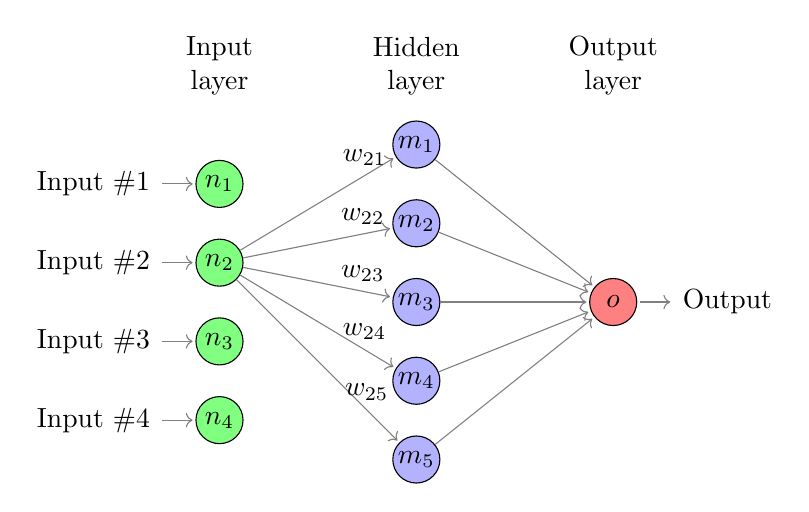
\begin{tikzpicture}[shorten >=1pt,->,draw=black!50, node distance=\layersep]
%https://tex.stackexchange.com/questions/96846/how-to-place-label-in-middle-of-line-above-and-below-with-tikz
    \tikzstyle{every pin edge}=[<-,shorten <=1pt]
    \tikzstyle{neuron}=[circle,fill=black!25,minimum size=17pt,inner sep=0pt, draw=black]
    \tikzstyle{input neuron}=[neuron, fill=green!50];
    \tikzstyle{output neuron}=[neuron, fill=red!50];
    \tikzstyle{hidden neuron}=[neuron, fill=blue!30];
    \tikzstyle{annot} = [text width=4em, text centered]

    % Draw the input layer nodes
    \foreach \name / \y in {1,...,4}
    % This is the same as writing \foreach \name / \y in {1/1,2/2,3/3,4/4}
        \node[input neuron, pin=left:Input \#\y] (I-\name) at (0,-\y) {$n_\y$};

    % Draw the hidden layer nodes
    \foreach \name / \y in {1,...,5}
        \path[yshift=0.5cm]
            node[hidden neuron] (H-\name) at (\layersep,-\y cm) {$m_\y$};

    % Draw the output layer node
    \node[output neuron,pin={[pin edge={->}]right:Output}, right of=H-3] (O) {$o$};

    % Connect every node in the input layer with every node in the
    % hidden layer.
%    \foreach \source in {1,...,4}
%        \foreach \dest in {1,...,5}
%            \draw (I-\source) -- node[below] {$w_ij$} ++ (H-\dest);


%    \foreach \source in {1,...,4}
        \foreach \dest in {1,...,5}
            \draw (I-2) -- node[above, pos=0.8] {$w_{2\dest}$} ++ (H-\dest);

    % Connect every node in the hidden layer with the output layer
    \foreach \source in {1,...,5}
        \path (H-\source) edge (O);

    % Annotate the layers
    \node[annot,above of=H-1, node distance=1cm] (hl) {Hidden layer};
    \node[annot,left of=hl] {Input layer};
    \node[annot,right of=hl] {Output layer};
\end{tikzpicture}
  \end{minipage}
  \vfill
\begin{minipage}[t][0.5\textheight][t]{\textwidth}

\end{minipage}


\end{frame}







\begin{frame}[fragile]{Point Variance of Linear Predictor}

\begin{align*}
\action<+->{ &=&&}
\\
\action<+->{  &=   && }
\end{align*}
\action<+->{The}
\end{frame}



\begin{frame}[fragile]{Correlation}
\begin{itemize}
\item[] \textbf{Serial No.} is basically uncorrelated with anything. \pause
\item[] \textbf{Admit} is highly correlated with \textbf{CGPA}, \textbf{TOEFL Score} and \textbf{GRE Score}\pause
\item[] \textbf{Research} has a lowish correlation with \textbf{Admit}, but also with everything else.  
\end{itemize}
\end{frame}











\begin{frame}[fragile]{Bias, Variance and Parameters}
  \begin{minipage}[t][0.5\textheight][t]{\textwidth}
	\centering
	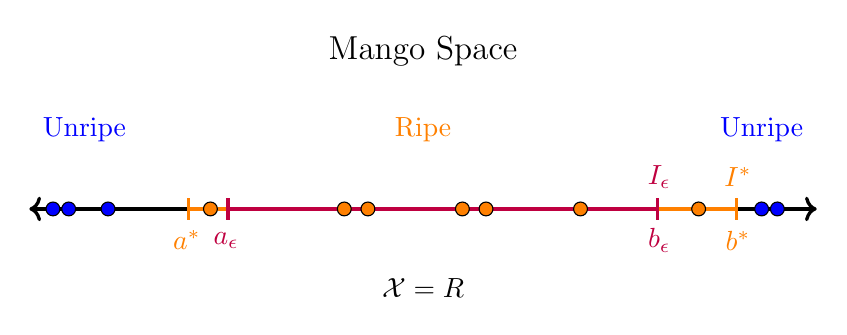
\begin{tikzpicture}
		\draw[<->,very thick] (-5,0) -- (5,0);
		\draw[color = orange, |-|,very thick] (-3,0) -- (4,0);
		\node[color=orange] at (4,.4) {$I^*$};
		\node at (0,2) {\large Mango Space} ;
		\node at (0,-1) {$\mathcal{X} = \mathbb{R}$} ;
		\node [color=blue] at (-4.3,1) {Unripe} ;
		\node [color=blue] at (4.3,1) {Unripe} ;
		\node [color=orange] at (0,1) {Ripe} ;

		\node [color=orange] at (-3,-.4) {$a^*$} ;
		\node [color=orange] at (4,-.4) {$b^*$} ;

		\draw [color=purple, |-|,very thick] (-2.5,0) -- (3,0);
		\node [color=purple] at (3,.4) {$I_\epsilon$} ;
		\node [color=purple] at (-2.5,-.4) {$a_\epsilon$} ;
		\node [color=purple] at (3,-.4) {$b_\epsilon$} ;

%		\draw [color=olive, |-|,very thick] (-3.5,0) -- (2.5,0);
%		\node [color=olive] at (3,.4) {$h_{\mathcal{T}}$} ;



		\node[circle,draw=black, fill=orange, inner sep=0pt,minimum size=5pt] at (2,0) {};
		\node[circle,draw=black, fill=orange, inner sep=0pt,minimum size=5pt] at (-1,0) {};
		\node[circle,draw=black, fill=orange, inner sep=0pt,minimum size=5pt] at (-.7,0) {};
		\node[circle,draw=black, fill=orange, inner sep=0pt,minimum size=5pt] at (.5,0) {};
		\node[circle,draw=black, fill=orange, inner sep=0pt,minimum size=5pt] at (.8,0) {};
		\node[circle,draw=black, fill=orange, inner sep=0pt,minimum size=5pt] at (-2.7,0) {};
		\node[circle,draw=black, fill=orange, inner sep=0pt,minimum size=5pt] at (3.5,0) {};

		\node[circle,draw=black, fill=blue, inner sep=0pt,minimum size=5pt] at (-4.5,0) {};
		\node[circle,draw=black, fill=blue, inner sep=0pt,minimum size=5pt] at (-4,0) {};
		\node[circle,draw=black, fill=blue, inner sep=0pt,minimum size=5pt] at (-4.7,0) {};
		\node[circle,draw=black, fill=blue, inner sep=0pt,minimum size=5pt] at (4.3,0) {};
		\node[circle,draw=black, fill=blue, inner sep=0pt,minimum size=5pt] at (4.5,0) {};
	\end{tikzpicture}
  \end{minipage}
  \vfill
  \begin{minipage}[t][0.5\textheight][t]{\textwidth}
Lets understand this visually.
$$
Err(x_0) = \sigma_\epsilon^2 + [E_\cT[\hat f(x_0)] - f(x_0)]^2 + E_\cT\big[ \hat{f}(x_0) - E_\cT[\hat{f}(x_0)] \big]^2\,.
$$\pause
Consider a data set, 
\end{minipage}
\end{frame}





























